\chapter{Overview}

\prettyref{fig:Kerberose-block-diagram-overview} shows a high-level overview of the Kerberos processor.

\begin{figure}
% Kerberos overview, similar to Taiga diagram
    \begin{center}
        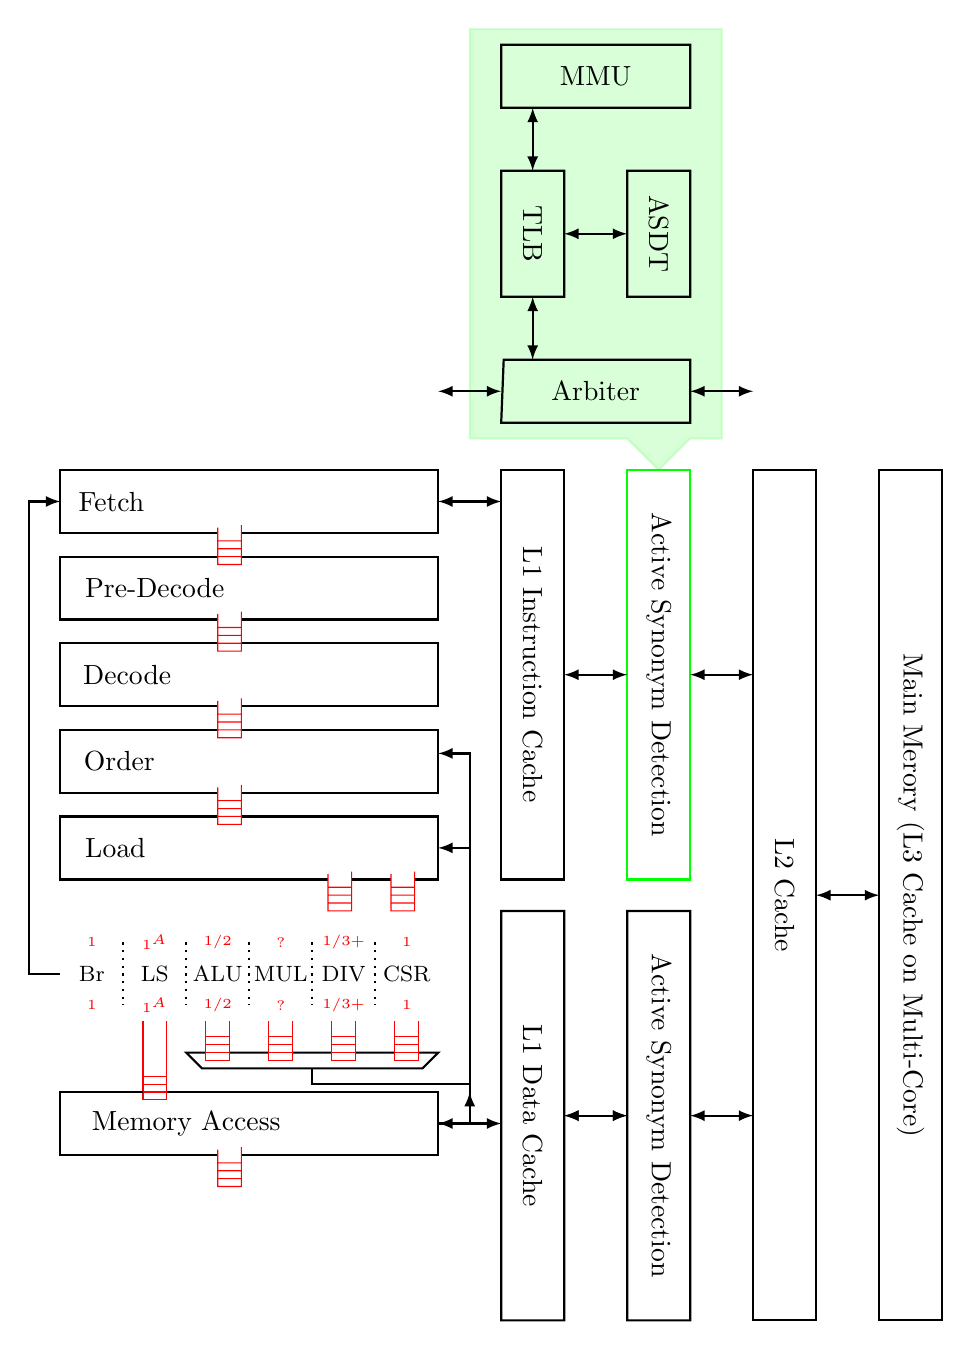
\begin{tikzpicture}[scale=0.2]
            \tikzstyle{every node}+=[inner sep=0pt]

            % Fetch
            \path
                 % Outer rectangle
                 [black,draw,thick]
                 % Origin
                 (0,0) node [black] (Fetch) {}
                 % Label
                 (Fetch) ++(3.25,-2) node [black] {Fetch}
                 % Box
                 (Fetch)
               ++(10,-4) -- ++(-10,0) -- ++(0,4) -- ++(24,0) -- ++(0,-4) -- ++(-12.5,0)
                 % Pipeline position
                 (Fetch) ++(10,-3.5) node (FetchPL1) {};

            % Pre-Decoder
            \path
                [black, draw, thick]
                % Origin, relative to Fetch
                (Fetch) ++(0,-5.5) node (PreDecode) {}
                (PreDecode) ++(6,-2) node {Pre-Decode}
                % Box
                (PreDecode)
                (FetchPL1) ++(0,-2)
                -- ++(-10,0) -- ++(0,-4) -- ++(10,0)
              ++(1.5,0) -- ++(12.5,0) -- ++(0,4) -- ++(-12.5,0)
                (PreDecode) ++(10,-3.5) node (PreDecodePL1) {};

            % Decoder
            \path
                [black, draw, thick]
                % Origin, relative to Fetch
                (PreDecode) ++(0,-5.5) node (Decode) {}
                (Decode) ++(4.25,-2) node {Decode}
                % Box
                (Decode)
                (PreDecodePL1) ++(0,-2)
                -- ++(-10,0) -- ++(0,-4) -- ++(10,0)
              ++(1.5,0) -- ++(12.5,0) -- ++(0,4) -- ++(-12.5,0)
                (Decode) ++(10,-3.5) node (DecodePL1) {};

            % Ordering
            \path
                [black, draw, thick]
                % Origin, relative to Fetch
                (Decode) ++(0,-5.5) node (Order) {}
                (Order) ++(3.75,-2) node {Order}
                % Box
                (Order)
                (DecodePL1) ++(0,-2)
                -- ++(-10,0) -- ++(0,-4) -- ++(10,0)
              ++(1.5,0) -- ++(12.5,0) -- ++(0,4) -- ++(-12.5,0)
                (Order) ++(10,-3.5) node (OrderPL1) {};

            % Load
            \path
                [black, draw, thick]
                (Order) ++(0,-5.5) node (Load) {}
                (Load) ++(3.5,-2) node {Load}
                (OrderPL1) ++(0,-2)
              -- ++(-10,0) -- ++(0,-4) -- ++(17,0)
              ++(0,0.5) node (LoadPL1) {}
              ++(1.5,-0.5) -- ++(2.5,0) ++(0,0.5) node (LoadPL2) {}
              ++(1.5,-0.5) -- ++(1.5,0) -- ++(0,4) -- ++(-12.5,0);

            %%%%%%%%%%%%%%%%%
            % Execute phase %
            %%%%%%%%%%%%%%%%%

            \path (Load) ++(0,-8) node (ExecutePhase) {};

            \path
                [black, draw, thick, text centered]
                (ExecutePhase) node (ExBranch) {}
              ++(2,-2) node {\footnotesize{Br}}
                (ExBranch) ++(2,0) node [red] {\tiny{1}}
              ++(0,-4) node [red] {\tiny{1}};
            \path
                [black, draw, thick, text centered]
                (ExBranch) ++(4,0) node (ExLS) {}
              ++(2,-2) node {\footnotesize{LS}}
                (ExLS) ++(2,0) node [red] {\tiny{$1^A$}}
              ++(0,-4) node [red] {\tiny{$1^A$}};
            \path
                [black, draw, thick, text centered]
                (ExLS) ++(4,0) node (ExALU) {}
              ++(2,-2) node {\footnotesize{ALU}}
                (ExALU) ++(2,0) node [red] {\tiny{1/2}}
              ++(0,-4) node [red] {\tiny{1/2}};
            \path
                [black, draw, thick, text centered]
                (ExALU) ++(4,0) node (ExMUL) {}
              ++(2,-2) node {\footnotesize{MUL}}
                (ExMUL) ++(2,0) node [red] {\tiny{?}}
              ++(0,-4) node [red] {\tiny{?}};
            \path
                [black, draw, thick, text centered]
                (ExMUL) ++(4,0) node (ExDIV) {}
              ++(2,-2) node {\footnotesize{DIV}}
                (ExDIV) ++(2,0) node [red] {\tiny{1/3+}}
              ++(0,-4) node [red] {\tiny{1/3+}};
            \path
                [black, draw, thick, text centered]
                (ExDIV) ++(4,0) node (ExCSR) {}
              ++(2,-2) node {\footnotesize{CSR}}
                (ExCSR) ++(2,0) node [red] {\tiny{1}}
              ++(0,-4) node [red] {\tiny{1}};
            \path
                [black, draw, thick, dotted]
                (ExBranch)
              ++(4,0) -- ++(0,-4)
                (ExLS)
              ++(4,0) -- ++(0,-4)
                (ExALU)
              ++(4,0) -- ++(0,-4)
                (ExMUL)
              ++(4,0) -- ++(0,-4)
                (ExDIV)
              ++(4,0) -- ++(0,-4);
            % Mux
            \path
                [black, draw, thick]
                (ExALU) ++(1.25,-7)
                node (ExMux) {}
              ++(1.5,0) -- ++(2.5,0)
              ++(1.5,0) -- ++(2.5,0)
              ++(1.5,0) -- ++(2.5,0)
              ++(1.5,0) -- ++(1.25,0)
                -- ++(-1,-1) -- ++(-14,0) -- ++(-1,1) -- ++(1.25,0);
            % Execution unit pipelines
            \foreach \x in {ExALU, ExMUL, ExDIV, ExCSR}
            \path
                [red, draw]
                (\x) ++(1.25,-5) -- ++(0,-2.5) -- ++(1.5,0) -- ++(0,2.5)
                (\x) ++(1.25,-5) -- ++(0,-2) -- ++(1.5,0)
              ++(0,0.5) -- ++(-1.5,0)
              ++(0,0.5) -- ++(1.5,0);

            % LS has a longer reach to the MEM stage
            \path
                [red, draw]
                (ExLS) ++(1.25,-5) -- ++(0,-5) -- ++(1.5,0) -- ++(0,5)
                (ExLS) ++(1.25,-7.5) -- ++(0,-2) -- ++(1.5,0)
              ++(0,0.5) -- ++(-1.5,0)
              ++(0,0.5) -- ++(1.5,0);
            % Branch and forward
            \path
                [->,>=latex,black,draw,thick]
                (ExMux) ++(6.75,-1)
                -- ++(0,-1) -- ++(10,0) -- ++(0,15) -- ++(-2,0);
            \path
                [->,>=latex,black,draw,thick]
                (ExMux) ++(6.75,-1) ++(10,14)
                -- ++(0,6) -- ++(-2,0);
            \path
                [->,>=latex,black,draw,thick]
                (ExBranch) ++(0,-2)
                -- ++(-2,0) -- ++(0,30) -- ++(2,0);
            % Mem
            \path
                [black, draw, thick]
                % Origin, relative to Exec
                (ExecutePhase) ++(0,-9.5) node (MemPhase) {}
                (MemPhase) ++(8,-2) node {Memory Access}
                % Box
                (ExLS) ++(1.25,-9.5) -- ++(-5.25,0)
                -- ++(0,-4) -- ++(10,0)
              ++(1.5,0) -- ++(12.5,0) -- ++(0,4) -- ++(-17.25,0)
                (MemPhase) ++(10,-3.5) node (MemPL1) {};
            \path
                [->,>=latex,black,draw,thick]
                (MemPhase) ++(24,-2)
                -- ++(2,0) -- ++(0,4)
              ++(0,-4) -- ++(0,2);
            % Pipelines
            \foreach \x in {FetchPL1, PreDecodePL1, DecodePL1, OrderPL1, LoadPL1, LoadPL2, MemPL1}
            \path
                [red, draw]
                (\x) -- ++(0,-2.5) -- ++(1.5,0) -- ++(0,2.5)
                (\x) ++(0,-2) -- ++(1.5,0)
                ++(0,0.5) -- ++(-1.5,0)
                ++(0,0.5) -- ++(1.5,0);
            %%%%%%%%%%%%%%%%%%
            % Memory Systems %
            %%%%%%%%%%%%%%%%%%

            % L1 I$
            \path
                [black, draw, thick]
                (Fetch) ++(28,0) node (ICache) {}
              ++(2,-13) node [rotate=-90] {L1 Instruction Cache}
                (ICache)
                -- ++(4,0) -- ++(0,-26) -- ++(-4,0) -- ++(0,26) -- cycle;
            \path
                [<->,>=latex,black,draw,thick]
                (Fetch) ++(24,-2) -- ++(4,0);
            % Active Synonym Detection layer
            \path
                [green, draw, thick]
                (ICache) ++(8,0) node (IASD) {}
              ++(2,-13) node [black,rotate=-90] {Active Synonym Detection}
                (IASD)
                -- ++(4,0) -- ++(0,-26) -- ++(-4,0) -- ++(0,26) -- cycle;
            \path
                [<->,>=latex,black,draw,thick]
                (ICache) ++(4,-13) -- ++(4,0);
            % ASD Expansion
            \path
                [fill, draw, thick, green, opacity=0.15]
                (ICache) ++(-1,28) node (IASD Detail) {}
                (IASD Detail) ++(11,-28)
                -- ++(-2,2) -- ++(-10,0) -- ++(0,26) -- ++(16,0) -- ++(0,-26) -- ++(-2,0) -- cycle;
            \path
                [black, draw, thick]
                (IASD Detail) ++(1,-21) node (IASD Arbiter) {}
              ++(6,-2) node {Arbiter}
                (IASD Arbiter)
                -- ++(12,0) -- ++(0,-4) -- ++(-12,0) -- cycle;
            \path
                [black, draw, thick]
                (IASD Arbiter) ++(0,12) node (TLB) {}
              ++(2,-4) node [rotate=-90] {TLB}
                (TLB)
                -- ++(4,0) -- ++(0,-8) -- ++(-4,0) -- ++(0,8) -- cycle;
            \path
                [black, draw, thick]
                (TLB) ++(8,0) node (ASDT) {}
              ++(2,-4) node [rotate=-90] {ASDT}
                (ASDT)
                -- ++(4,0) -- ++(0,-8) -- ++(-4,0) -- ++(0,8) -- cycle;
            \path
                [black, draw, thick]
                (TLB) ++(0,8) node (MMU) {}
              ++(6,-2) node {MMU}
                (MMU)
                -- ++(12,0) -- ++(0,-4) -- ++(-12,0) -- ++(0,4) -- cycle;

            \path
                [<->,>=latex,black,draw,thick]
                (IASD Arbiter) ++(-4,-2) -- ++(4,0);
            \path
                [<->,>=latex,black,draw,thick]
                (IASD Arbiter) ++(12,-2) -- ++(4,0);
            \path
                [<->,>=latex,black,draw,thick]
                (IASD Arbiter) ++(2,0) -- ++(0,4);
            \path
                [<->,>=latex,black,draw,thick]
                (TLB) ++(4,-4) -- ++(4,0);
            \path
                [<->,>=latex,black,draw,thick]
                (TLB) ++(2,0) -- ++(0,4);

            % L1 D$
            \path
                [black, draw, thick]
                (ICache) ++(0,-28) node (DCache) {}
              ++(2,-13) node [rotate=-90] {L1 Data Cache}
                (DCache)
                -- ++(4,0) -- ++(0,-26) -- ++(-4,0) -- ++(0,26) -- cycle;
                \path
                [<->,>=latex,black,draw,thick]
                (DCache) ++(4,-13) -- ++(4,0);
            \path
                [<->,>=latex,black,draw,thick]
                (MemPhase) ++(24,-2) -- ++(4,0);
            % Active Synonym Detection layer
            \path
                [black, draw, thick]
                (DCache) ++(8,0) node (DASD) {}
              ++(2,-13) node [rotate=-90] {Active Synonym Detection}
                (DASD)
                -- ++(4,0) -- ++(0,-26) -- ++(-4,0) -- ++(0,26) -- cycle;
                \path
                [<->,>=latex,black,draw,thick]
                (DCache) ++(4,-13) -- ++(4,0);

            % L2 Cache
            \path
                [black, draw, thick]
                (IASD) ++(8,0) node (L2 Cache) {}
              ++(2,-27) node [rotate=-90] {L2 Cache}
                (L2 Cache)
                -- ++(4,0) -- ++(0,-54) -- ++(-4,0) -- ++(0,54) -- cycle;
            \path
                [<->,>=latex,black,draw,thick]
                (IASD) ++(4,-13) -- ++(4,0);
            \path
                [<->,>=latex,black,draw,thick]
                (DASD) ++(4,-13) -- ++(4,0);
            % L3 Cache
            \path
                [black, draw, thick]
                (L2 Cache) ++(8,0) node (L3 Cache) {}
                ++(2,-27) node [rotate=-90] {Main Merory (L3 Cache on Multi-Core)}
                (L3 Cache)
                -- ++(4,0) -- ++(0,-54) -- ++(-4,0) -- ++(0,54) -- cycle;
            \path
                [<->,>=latex,black,draw,thick]
                (L2 Cache) ++(4,-27) -- ++(4,0);
        \end{tikzpicture}
    \end{center}
    \label{fig:Kerberose-block-diagram-overview}
\end{figure}

\section{Memory Access and Cache}

Both \inlinecode{MemoryAccess} and \inlinecode{Fetch} connect directly to VC-DSR L1 cache.   L1 is virtually-indexed, virtually-tagged (VIVT); L2 and beyond are physically-indexed, physically-tagged (PIPT).  I\$ and D\$ use separate Active Synonym Detection Tables (ASDTs).

L1 only requires one cycle to access a cache line by its leading virtual address.  For potential active synonyms—comparatively rare—L1 requires two cycles if a full lookup through the Address Remapping Table (ART) adds enough time to put an L1 cache hit in the critical path.  This VC-DSR implementation uses last leading virtual page (LLVP) caching and ignores ASIDs for global pages to avoid ART look-ups via detecting them as homonyms.

On miss, L1 cache accesses an Active Synonym Detection (ASD) arbiter.  If the data is in L1 cache and the address remapping table (ART) does not include the virtual page as a synonym to the leading virtual page (LVP), the Translation Lookaside Buffer (TLB) and Active Synonym Detection Table (ASDT) provide this information and replay the cache request.  The TLB may perform a page table walk through the MMU during this process and check the resulting physical page against the ASDT.

When the ASDT does not contain a match, the ASD arbiter consults further memory systems, such as L2 cache or main memory.  Multi-core systems may use an L3 cache shared between cores; FPGA implementation may implement L2 or L3 on non-paging external RAM, such as 16Mib (2Mio) of 10ns static RAM arranged with 64-bit word size (around \$8).